\section{Data Scraping \& Processing}
\subsection{Process}
\begin{enumerate}
    \item{User provides input to the simple interface to set up a course.}
    \item{Input is sent to the server and starts the scraper module.}
    \item{Module scrapes the \code{HTML} from the provided webpages, and also follows forum links recursively to collect data of individual posts.}
    \item{Our custom data extraction algorithm filters the different structures on the page and extracts the relevant text.}
    \item{The data is analysed for keywords using the tf-idf algorithm.}
    \item{The data and its corresponding keywords are inserted into the database.}
    \item{An interactive model of the dataset appears on the webpage once the course is ready.}
    \item{Entities are updated automatically in Dialogflow to include new keywords, so our bot can recognise new requests from students}
\end{enumerate}

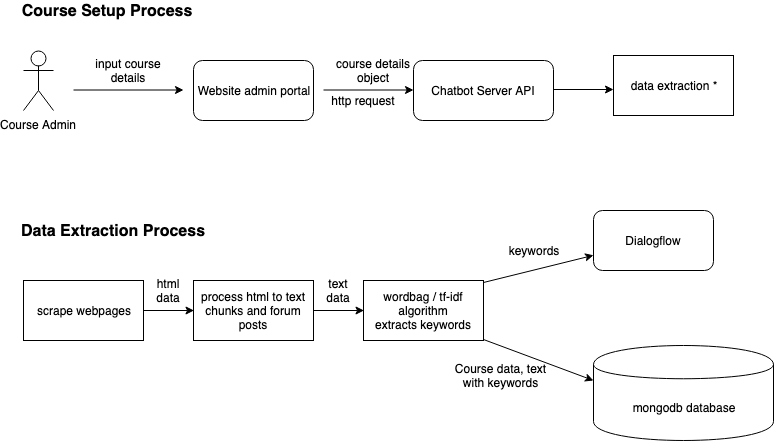
\includegraphics[width=\textwidth]{extraction.png}

\subsection{Example Usage}
This is an example use case based on the first user story described in section 2.1.2.

The course administrator registers an account, and then logs in via the front end. They are greeted with the setup dashboard, where they provide links to web pages that will be included in the bot's data set.

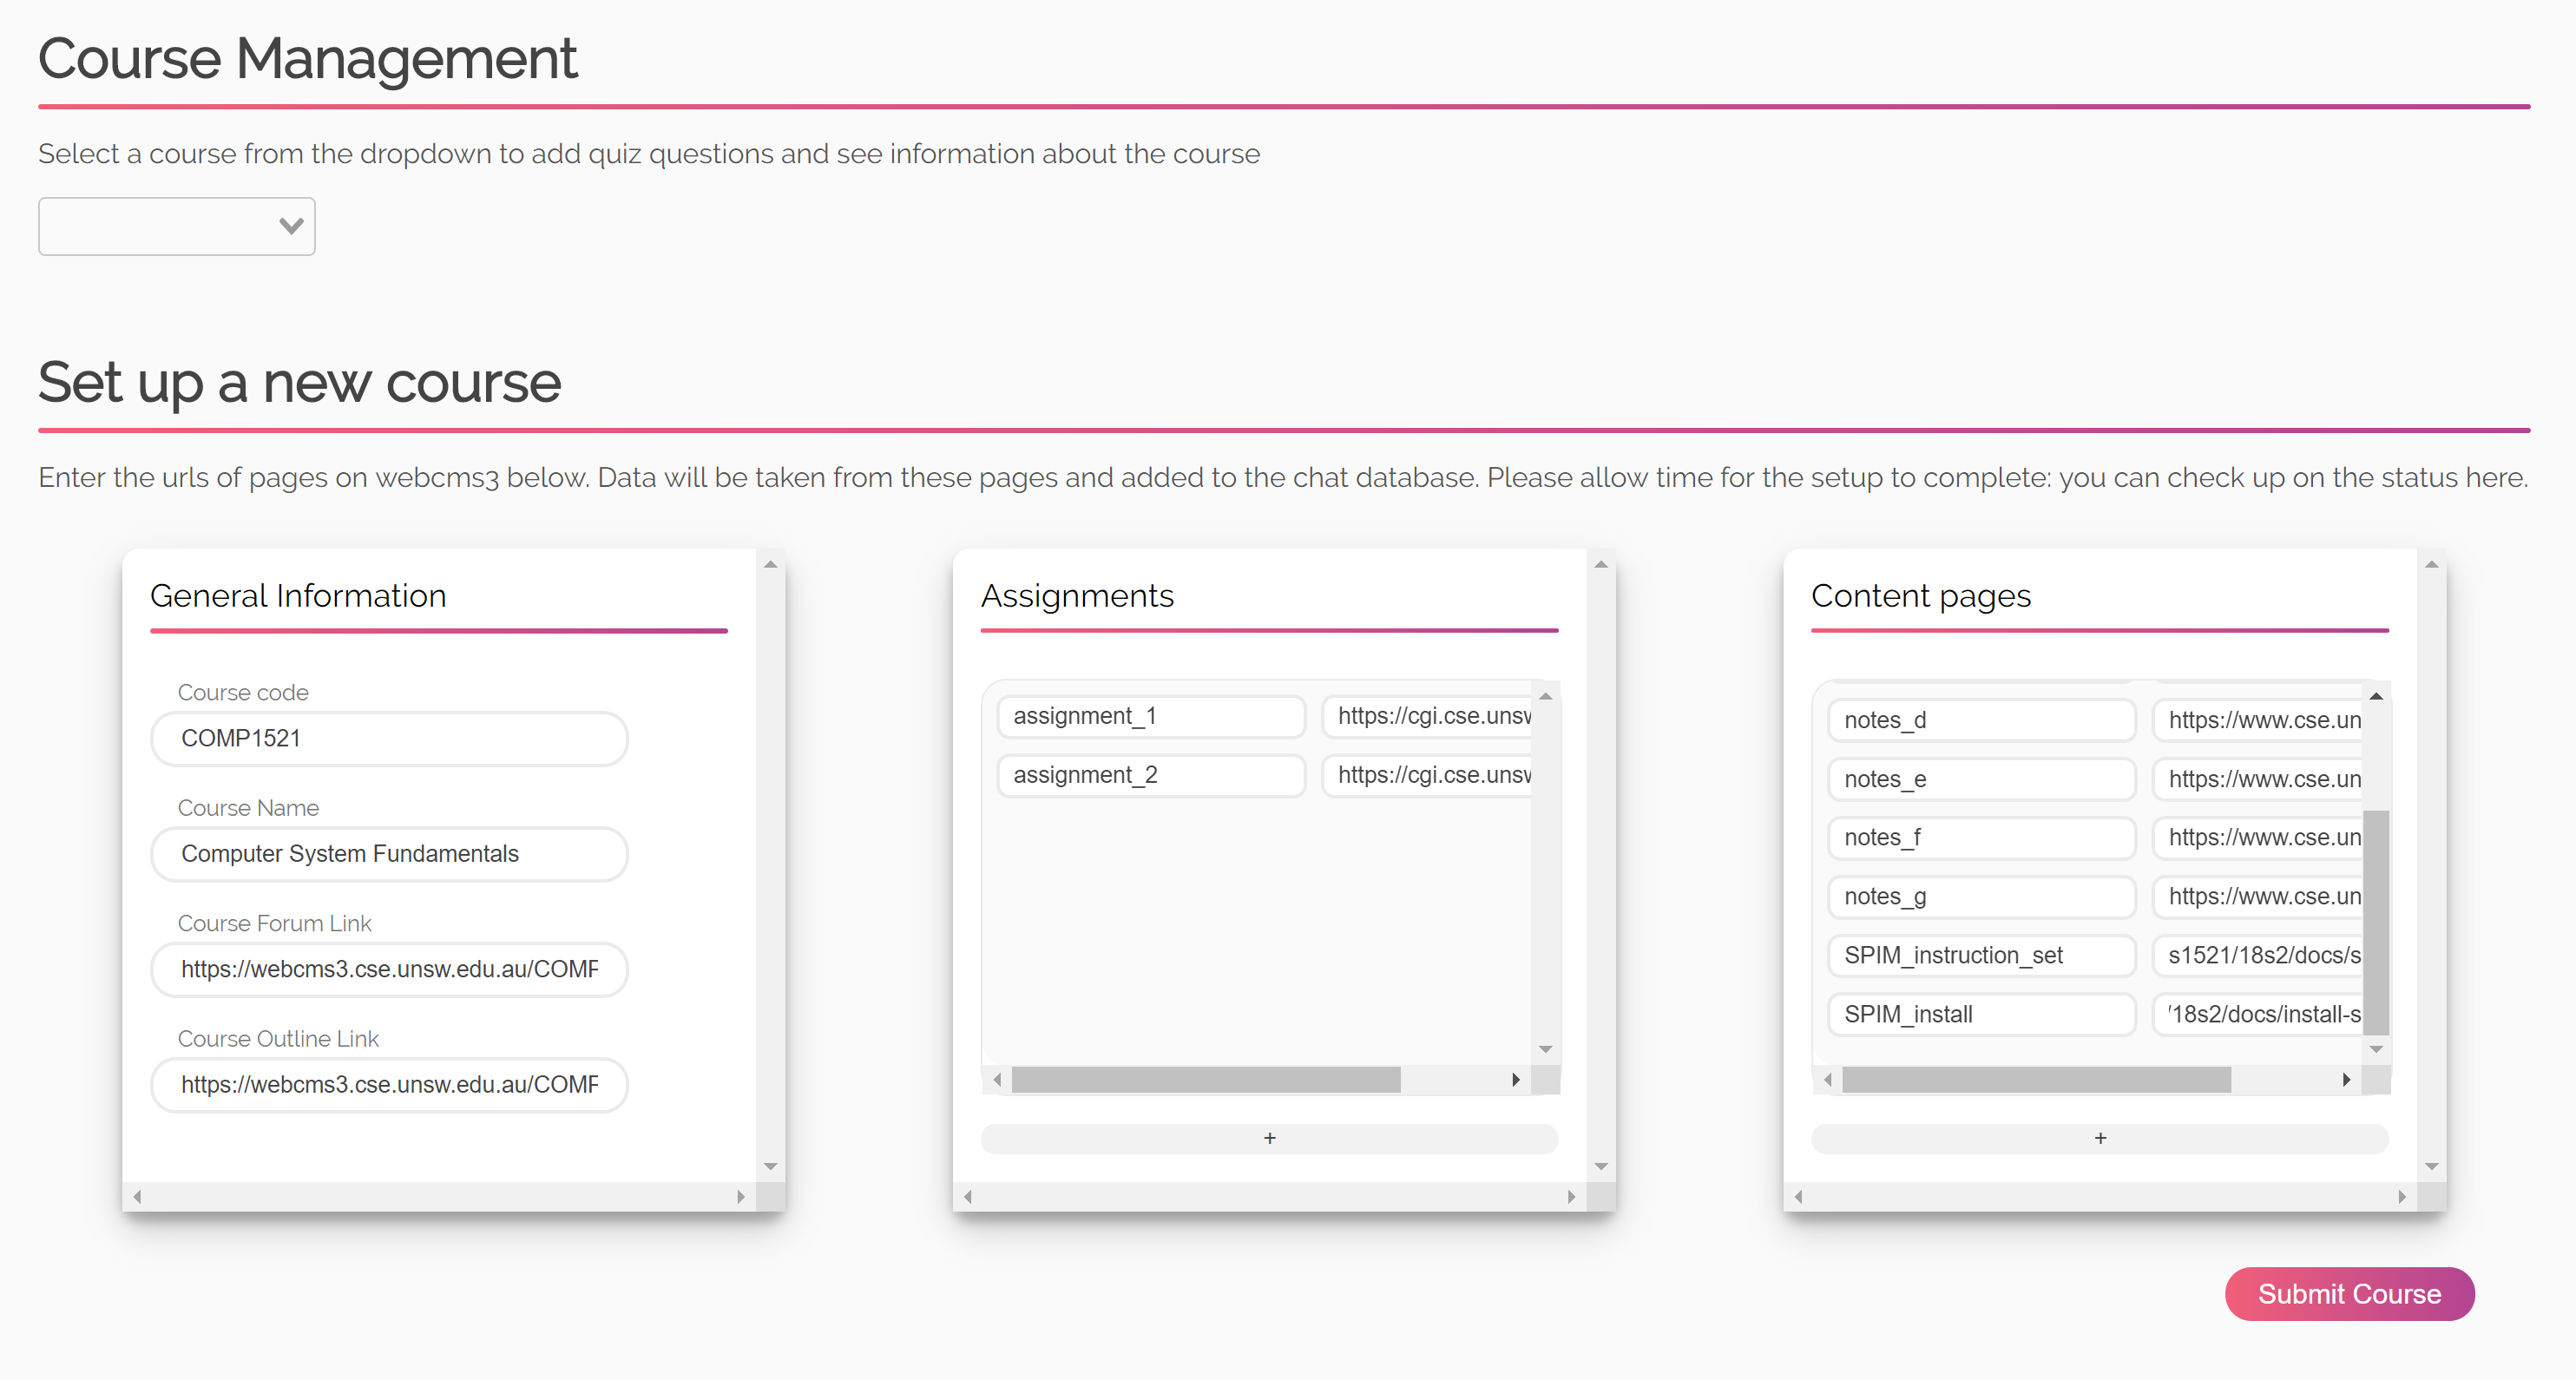
\includegraphics[width=\textwidth]{data-input.png}

Once the form is submitted, the data scraper module will process the pages and extract data. This data will be stored in the database and is ready for use.

\begin{center}
    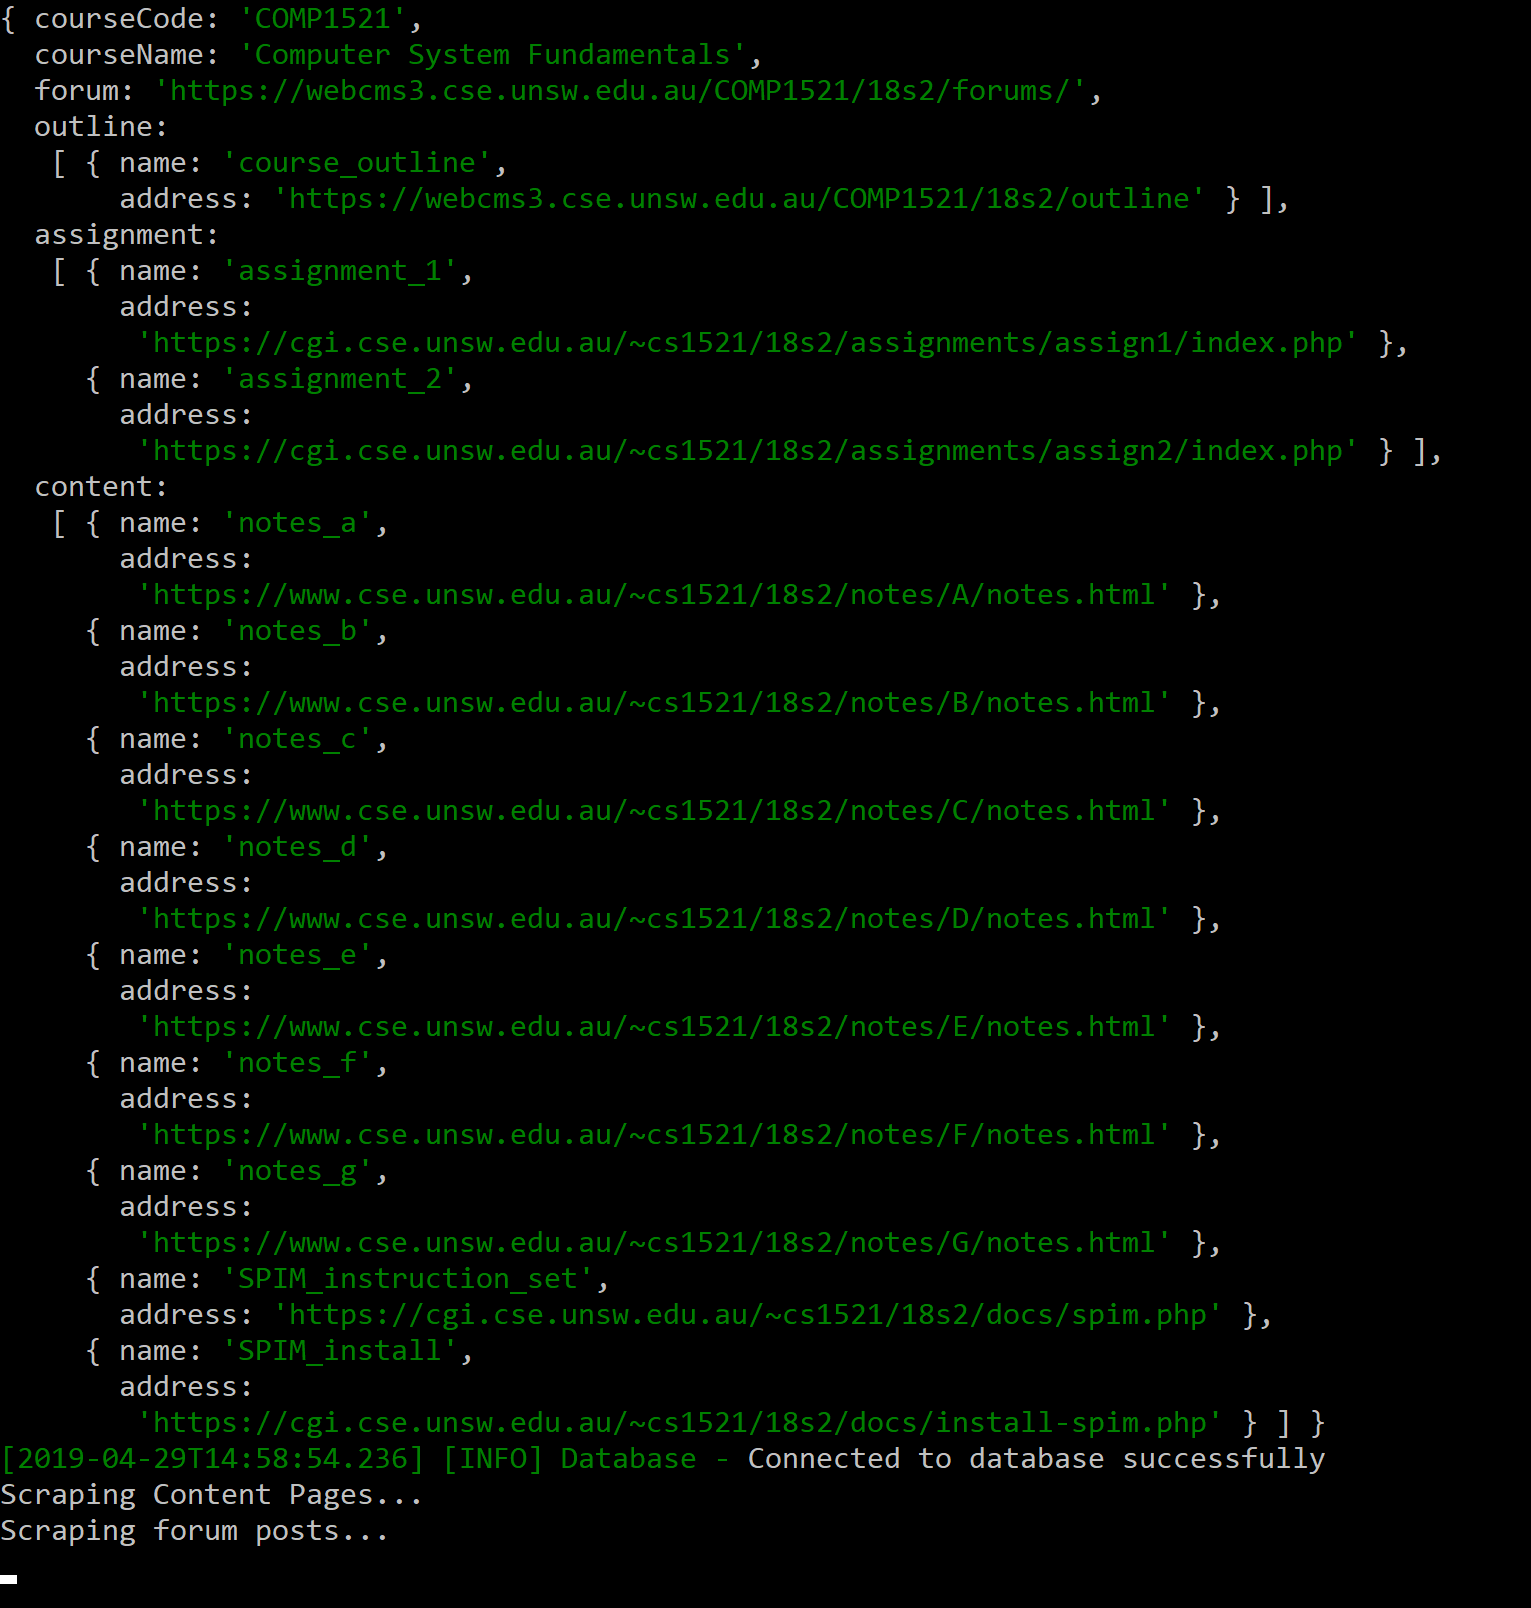
\includegraphics[width=10cm]{data-log.png}
\end{center}

\subsection{Technical Details}
The frontend is developed in \code{Vue.js} using \code{TypeScript}. This helps enforce data types within \code{JavaScript}, to ensure that the input sent to the backend is valid.

The server is created with \code{Node.js}. The data extraction makes use of asynchronous \code{Node.js} to reduce the amount of time spent in blocking processes such as api calls and filesystem/\code{http} calls. This is particularly important because it would otherwise cause the server to block and fail to process requests. Instead of having to spawn a new process, \code{Node.js} is able to manage all running processes and allow the data extraction module to run in the background.

We also use the \code{cheerio js} library, as it provides tools to parse \code{HTML} into usable data.

To extract tags (keywords) from text data, we used the bag of words model with the tf-idf algorithm. This generated tags by only considering the frequency of words in the entire set of text data, and allowed us to calculate the salience (importance) of each tag to each individual text data point. Each tag receives two scores: salience (the importance of the tag according to the tf-idf algorithm), and theta (a trainable value which is initialized as the same value as salience).

This was chosen over the Google Cloud NLP's keyword extraction module because the latter occasionally missed important tags, and also because it calculated the salience such that the sum of one data point will be one. This is not ideal for our system, as long sentences will tend to have a lower salience and be less likely to be presented to users. Instead, the tf-idf algorithm that we implemented suits our use case better, as it does not miss any tags for our data points, and also assigns a lower salience to common words, which helps us calculate accurate scores for each data point.


\code{MongoDB} is used for the database. It is the most appropriate software to handle the unstructured data that we deal with.

\newpage
